% !TeX spellcheck = el_GR-en_US
  \documentclass[11pt]{article}
  \usepackage{geometry}
  \geometry{a4paper, top=2.5cm, bottom=2.5cm, left=2.2cm,
    right=2.2cm}
  \usepackage{fontspec}
  \usepackage[nonumeralsign]{xgreek}
  \usepackage{fancyhdr}
  \usepackage{hyperref}
  \usepackage{enumitem}
  \usepackage{cite}
  \usepackage{multirow}
  \usepackage{float}
  \usepackage{graphicx}
  \usepackage{caption}
  \usepackage{amsmath}
  \usepackage{ifpdf}
  \usepackage{mathtools}
  \usepackage{siunitx}
  \usepackage{subfig}
  \usepackage{xfrac}
  \usepackage{booktabs}
  \usepackage{blindtext}
  \usepackage{array}
  \usepackage{amsmath}



  \setmainfont{Baskerville}
  \setmonofont{Consolas}

  \graphicspath{ {./images/} }
  
  \newcommand{\ypertitlos}{Εργασία στο μάθημα Βάσεις Δεδομένων}
  \newcommand{\titlos}{EventDB}
  \newcommand{\ypotitlos}{Βάση δεδομένων για εκδηλώσεις}
  \newcommand{\paradoteo}{1ο Παραδοτέο}
  \newcommand{\omada}{Ομάδα 14}
  \newcommand{\student}[3]{#1&#2&#3\\}
  \newcommand{\melosA}{\student{Μπλάννινγκ Φρανκ}{6689}{frankgou@auth.gr}}
  \newcommand{\melosB}{\student{Θεοδωρίδου Χριστίνα}{8055}{christtk@auth.gr}}
  \newcommand{\melosC}{\student{Ζησης Μηλης Εμμανουηλ}{8053}{zemmanox@auth.gr}}
  \newcommand{\hmnia}{\today}

  
  
  \pagestyle{fancy}
  \lhead{Βάσεις Δεδομένων 2018}
  \rhead{\titlos}
  \renewcommand{\headrulewidth}{0.4pt}
  \renewcommand{\footrulewidth}{0.4pt}
  \setlength{\headheight}{14pt}

  \hypersetup{colorlinks=true, linkcolor=black, urlcolor=blue, citecolor=blue}
  \urlstyle{same}

  \begin{document}
  \thispagestyle{empty}
  {\centering
    \Large\ypertitlos\\
    \vspace{7cm}
    \Huge\titlos\\
    \Large\ypotitlos\\
    \vspace{2cm}
  }
  \hfill \paradoteo

  \begin{figure}[H]
  \centering
  \includegraphics[width=\linewidth]{images/front.eps}
\end{figure}
  
  \vspace{8cm}
  \begin{tabular}[b]{l l l}
    \omada&&\\
    \melosA
    \melosB 
    \melosC
  \end{tabular}
  
  {\centering
    \vspace{2cm}
    \hmnia\\
  }
  \newpage

  \tableofcontents
  \listoffigures

  \newpage
  
  \section{Εισαγωγή}

\subsection{Σκοπός Εφαρμογής}

Οι σύγχρονες πόλεις, καθημερινά, δίνουν την δυνατότητα σε πολλούς
καλλιτέχνες και μη, να προβάλουν την δουλειά τους μέσω εκθέσεων,
συναυλιών ή άλλων εκδηλώσεων. Επίσης, καθημερινά διάφοροι οργανισμοί
και ομάδες διοργανώνουν διάφορες δραστηριότητες προς υποστήριξη και
ενημέρωση του κόσμου για τον σκοπό τους.

Αποτέλεσμα όλων αυτών είναι, στην σημερινή κοινωνία, τα δρώμενα που
λαμβάνουν χώρα καθημερινά να είναι πολυπληθή. Έτσι είναι απαραίτητη
μια εφαρμογή όπου θα περιέχει πληροφορίες για όλες αυτές τις
εκδηλώσεις έτσι ώστε να μπορούν οι ενδιαφερόμενοι να βρίσκουν τις
δραστηριότητες που τους ενδιαφέρουν. Μία τέτοια εφαρμογή απαιτεί μία
βάση δεδομένων για την αποθήκευση, προσπέλαση και επεξεργασία των
Πληροφοριών κάθε εκδήλωσης λόγο του μεγάλου όγκου της πληροφορίας
αυτής και την ανάγκη για παράλληλη επεξεργασία δεδομένων από πολλούς
χρήστες.

\subsection{Περιγραφή Εφαρμογής}

Συγκεκριμένα, στη δική μας εφαρμογή, εκος από τοποθεσία, είδος και
ημερομηνία της εκδήλωσης, ο χρήστης θα μπορεί να αγοράσει εισιτήρια
εκδηλώσεων ή να βρει φυσικά καταστήματα προπώλησης, να αποθηκεύσει
εκδηλώσεις που τον ενδιαφέρουν ώστε να τις δει αργότερα και άλλα. Όλα
αυτά είναι εφικτά λόγο της προσεκτικής σχεδίασης της βάσης δεδομένων
πίσω από την εφαρμογή

Για την βάση \titlos, τα δεδομένα, που θα αποθηκεύονται είναι το όνομα
των εκδηλώσεων, το είδος τους, οι ημερομηνίες διεξαγωγής τους, η
τοποθεσία που πραγματοποιούνται κτλ. Τη βάση θα μπορεί αν την
χρησιμοποιήσει ο οποιοσδήποτε, αρκεί να έχει πρόσβαση σε αυτήν μέσω
του διαδικτύου, στον ιστότοπο στον οποίο θα βρίσκεται. Επίσης, όποιος
θα ήθελε η εκδήλωσή του να δημοσιοποιηθεί, θα μπορεί συμπληρώνοντας
μια φόρμα εγγραφής να αποκτήσει πρόσβασή στην πλατφόρμα δημιουργίας
εκδήλωσης και να προστεθεί η εκδήλωση του στον ιστότοπο.

\subsection{Απαιτήσεις Εφαρμογής σε Δεδομένα}

Για την βάση \titlos, αναμένεται να έχουμε ~1050 κωδικούς εκδηλώσεων
(πχ για έναν μήνα) , που σημαίνει ~35 κωδικοί εκδηλώσεων κάθε
μέρα. Επίσης, αναμένεται οι ~20 να είναι μουσικής, οι ~25 να είναι
κάτα μέσο όρο απογευματινές ώρες κτλ



%%% Local Variables:
%%% mode: latex
%%% TeX-master: "main"
%%% End:

  
\section{Κατηγορίες Χρηστών και απαιτήσεις τους}

Στην συγκεκριμένη εφαρμογή και κατ' επέκταση η βάση δεδομένων θα έχει
έναν διαχειριστή και τρεις χρήστες, τον "Διοργανωτή" τον "Μη
Εγγεγραμμένο Χρήστη" και τον "Χρήστη". Μόνο οι τρεις χρήστες ορίζονται
παρακάτω μιας και ο διαχειριστής της εφαρμογής και της βάσης δεδομένων
θα εκτελεί ενέργειες με αυτόνομο τρόπο πέρα των πλαισίων της
εφαρμογής.

\underline{Διοργανωτής:}

Ο Διοργανωτής, μετά από εγγραφή του στο σύστημα, η οποία εγκρίνεται
από τον διαχειριστή, πρέπει να έχει την δυνατότητα να εκτελεί όλες τις
απαραίτητες ενέργειες έτσι ώστε να καταχωρεί όλες τις απαραίτητες
πληροφορίες μιας εκδήλωσης όπως και να έχει πρόσβαση στην λίστα αγορών
για τις εκδηλώσεις όπου διαχειρίζεται. Αναλυτικά:
\begin{itemize}[noitemsep]
\item Προσθήκη νέας τοποθεσίας διεξαγωγής
\item Προσθήκη νέων σημείων προπόλησης
\item Προσθηκη νέας εκδήλωσης
\item Προβολή λίστας αγορών εκδήλωσης όπου οργανώνει
\end{itemize}

\underline{Μη εγγεγραμμένος χρήστης}

Ο μη εγγεγραμμένος χρήστης έχει την δυνατότητα να προβάλει με διάφορα
κριτήρια εύρεσης τις μελλοντικές εκδηλώσεις και να πραγματοποιήσει
εγγραφή
\begin{itemize}[noitemsep]
\item Πρόσβαση σε δεδομένα που αφορούν τις εκδηλώσεις, μετά απο
  σχετική αναζήτηση.
\item Εγγραφή χρήστη
\end{itemize}

\underline{Χρήστης:}

Ο Χρήστης μετά από εγγραφή του, η οποία ολοκληρώνεται αυτόματα, έχει
την επιπλέον δυνατότητα, πέρα του μη εγγεγραμμένου χρήστη, να εκτελεί
αγορά εισιτήριων για τις εκδηλώσεις που το υποστηρίζουν, όπως και να
αποθηκεύει εκδηλώσεις που των ενδιαφέρουν για να τις δει
αργότερα. Αναλυτικά:
\begin{itemize}[noitemsep]
\item Προσθήκη νέας κάρτας πληρωμής
\item Αγορά εισιτήριου εκδήλωσης
\item Προσθήκη και αφαίρεση εκδήλωσης στην λίστα ενδιαφερομένων
\item Προβολή εκδηλώσεων στην λίστα ενδιαφερομένων
\end{itemize}


%%% Local Variables:
%%% mode: latex
%%% TeX-master: "main"
%%% End:

  \section{Μοντέλο Οντοτήτων/Συσχετίσεων}

\subsection{Γενική Περιγραφή}

Οι οντότητες είναι : οι Εκδήλωση, η Τοποθεσία, η Ημερομηνία, ο Καλλιτέχνης - Διοργανωτής, η Αγορά Εισιτηρίων και η Προσβασιμότητα. Για κάθε εκδήλωση θα πρέεπι να καταγράφεται το όνομά της, το είδος της και το όνομα του καλλιτέχνη-διοργανωτή.
\\
\\
\underline{Υποθέσεις:}
\begin{itemize}[noitemsep]

\item Ο κωδικός εκδήλωσης είναι μοναδικός για κάθε εκδήλωση. Για παράδειγμα, εφόσον ο κωδικός 101 αντιστοιχεί σε μια συγκικριμένη εκδήλωση (ασχέτως καλλιτέχνη ή τοποθεσίας), την ημερομηνία 1/12/2018, τότε ο ίδιος κωδικός δεν μπορεί να είναι κωδικός καμίας άλλης εκδήλωσης.
\item Η διαφημίσεις μπορούν να γίνουν μόνο σε έναν τηλεοπτικό ή ραδιοφωνικό σταθμό για κάθε εκδήλωση. Επίσης θα υπάρχει μόνο ένα μέρος τοποθέτησης αφισών κάθε φορά.


\end{itemize}

\subsection{Καθορισμός Οντοτήτων}

Παρακάτω φαίνονται οι οντότητες της \titlos, η περιγραφή τους καθώς και κάποια γνωρίσματά τους.

\begin{center}
\begin{tabular}[]{|c | c|}
\hline
\textbf{Όνομα Οντότητας}   &  Event  \\ \hline 
\textbf{Περιγραφή}         &  Οντότητα που αποθηκεύονται οι εκδηλώσεις \\ \hline 
\textbf{Ιδιότητες}         &  Ισχυρή οντότητα \\  \hline               
\textbf{Γνωρίσματα}        &  \underline{Κωδικός εκδήλωσης} \\
           ~               &  Είδος εκδήλωσης \\
            ~              &  Ύπαρξη Εισιτηρίου \\
             ~             &  Κοινό που απευθύνεται \\
              ~            &  Σκοπός \\ 
                           &  Ημερομηνία \\
                           &  Ώρα \\
\hline
\hline
\textbf{Όνομα Οντότητας}   &  Location \\ \hline 
\textbf{Περιγραφή}         &  Οντότητα που αποθηκεύονται οι τοποθεσίες των εκδηλώσεων \\ \hline 
\textbf{Ιδιότητες}         &  Ασθενής οντότητα \\ \hline 
\textbf{Γνωρίσματα}        &  \underline{Κωδικός τοποθεσίας} \\
                           &  Όνομα \\
           ~               &  Οδός \\
             ~             &  ΤΚ\\
                           &  Εσωτερικός ή Εξωτερικός χώρος \\
                           &  Τηλέφωνο \\
                           & { \begin{tabular}[]{c|c}
                            Κάτάλογος τιμών           & μπύρα \\
                                                      & κρασί \\
                                                      & ποτό \\  
                           \end{tabular} }  
\\ \hline

\end{tabular}

\begin{tabular}[]{|c | c | } 
\hline
\textbf{Όνομα Οντότητας}   &  Artist \\ \hline 
\textbf{Περιγραφή}         &  Οντότητα που αποθηκεύονται οι καλλιτέχνες \\ \hline 
\textbf{Ιδιότητες}         &  Ισχυρή οντότητα    \\    \hline           
\textbf{Γνωρίσματα}        &  \underline{Κωδικός καλλιτέχνη}\\
                           &  Όνομα Καλλιτέχνη \\
           ~               &  Καταγωγή \\
            ~              &  Είδος \\
\hline 
\hline
\textbf{Όνομα Οντότητας}   &  Tickets \\ \hline 
\textbf{Περιγραφή}         &  Οντότητα που αποθηκεύονται οι τρόποι αγοράς εισιτηρίων \\\hline 
\textbf{Ιδιότητες}         &  Ασθενής οντότητα \\       \hline           
\textbf{Γνωρίσματα}        &  \underline{Κωδικός εκδήλωσης} \\
                          %  &  Ύπαρξη εισιτηρίου \\
                           &  Φυσικά καταστήματα προπώλησης \\
           ~               &  Ηλεκτρονικά καταστήματα προπώλησης \\
            ~              &  Εύρος τιμών \\
\hline 
\hline
\textbf{Όνομα Οντότητας}   &  Accessibility \\ \hline 
\textbf{Περιγραφή}         &  Οντότητα που αποθηκεύονται οι τρόποι πρόσβασης στην τοποθεσια \\ \hline 
\textbf{Ιδιότητες}         &  Ασθενής οντότητα \\  \hline                 
\textbf{Γνωρίσματα}        &  \underline{Κωδικός Τοποθεσίας} \\
                           &  Ύπαρξη χώρου στάθμευσης\\
            ~              &  Ύπαρξη κοντινών στάσεων \\
             ~             &  Ύπαρξη υποδομών για ΑΜΕΑ \\
                           & { \begin{tabular}[]{c|c}
                             Ύπαρξη τοποθεσιών με μισθωμένα ΜΜΜ           & τοποθεσία \\
                                                                         & ώρα \\ 
                           \end{tabular} }  
\\ \hline
\hline
\textbf{Όνομα Οντότητας}   &  Promotion \\ \hline 
\textbf{Περιγραφή}         &  Οντότητα που αποθηκεύονται οι τρόποι προώθησης της εκδήλωσης \\ \hline 
\textbf{Ιδιότητες}         &  Ασθενής οντότητα \\  \hline                 
\textbf{Γνωρίσματα}        &  \underline{Κωδικός Εκδήλωσης} \\
                           &  Ραδιοφωνικοί σταθμοί \\
            ~              &  Τηλεοπτικοί σταθμοί \\
             ~             &  Τοποθεσίες αφισών \\
                           & { \begin{tabular}[]{c|c}
                             Διαδικτυακή διαφήμηση & Κοινωνικά δίκτυα \\
                                                   & Ψηφιακές εφημερίδες \\
                                                   & Διάφορες ιστοσελίδες\\ 
                           \end{tabular} }  
\\ \hline
\hline
\textbf{Όνομα Οντότητας}   &  Communication \\ \hline 
\textbf{Περιγραφή}         &  Οντότητα που αποθηκεύονται οι τρόποι επικοινωνίας \\ \hline 
\textbf{Ιδιότητες}         &  Ασθενής οντότητα \\  \hline                 
\textbf{Γνωρίσματα}        &  \underline{Κωδικός Εκδήλωσης} \\
                           &  \underline{Όνομα Καλλιτέχνη} \\
            ~              &  Όνομα εταιρίας παραγωγής \\
             ~             &  email \\
                           &  Τηλέφωνο \\
\\ \hline
\end{tabular}
\end{center}


\subsection{Καθορισμός Συσχετίσεων}

Παρακάτω αναφέρονται οι συσχετίσεις της βάσης δεδομένων \titlos

\begin{tabular}[]{|p{4cm}|p{10cm}|}
  \hline
  \textbf{Όνομα Συσχέτισης} & Event\_Has\_Artist\\ \hline
  \textbf{Περιγραφή} & Κάθε εκδήλωση πρέπει να έχει 1 καλλιτέχνη\\ \hline
  \textbf{Ιδιότητες} & Has-A \{αναφέρετε αν είναι Is-A και αν είναι
                       Αναδρομική, Προσδιορίζουσα, Τριαδική\} \\ \hline
  \textbf{Λόγος πληθικότητας} & n:1 \\ \hline
  \textbf{Συμμετοχή} & Ολική Συμμετοχή του Event \\ \cline{2-2}
                     & Μερική Συμμετοχή του Artist \\ \hline
  \textbf{Γνωρίσματα} & - \\ \hline
\end{tabular}


\begin{tabular}[]{|p{4cm}|p{10cm}|}
  \hline
  \textbf{Όνομα Συσχέτισης} & Event\_Has\_Location\\ \hline
  \textbf{Περιγραφή} & Κάθε εκδήλωση πρέπει να έχει 1 τοποθεσία\\ \hline
  \textbf{Ιδιότητες} & Has-A \{αναφέρετε αν είναι Is-A και αν είναι
                       Αναδρομική, Προσδιορίζουσα, Τριαδική\} \\ \hline
  \textbf{Λόγος πληθικότητας} & n:1 \\ \hline
  \textbf{Συμμετοχή} & Ολική Συμμετοχή του Event \\ \cline{2-2}
                     & Μερική Συμμετοχή του Location \\ \hline
  \textbf{Γνωρίσματα} & - \\ \hline
\end{tabular}


\begin{tabular}[]{|p{4cm}|p{10cm}|}
  \hline
  \textbf{Όνομα Συσχέτισης} & Event\_Has\_Date\\ \hline
  \textbf{Περιγραφή} & Κάθε εκδήλωση πρέπει να έχει 1 ημερομηνία\\ \hline
  \textbf{Ιδιότητες} & Has-A \{αναφέρετε αν είναι Is-A και αν είναι
                       Αναδρομική, Προσδιορίζουσα, Τριαδική\} \\ \hline
  \textbf{Λόγος πληθικότητας} & n:1 \\ \hline
  \textbf{Συμμετοχή} & Ολική Συμμετοχή του Event \\ \cline{2-2}
                     & Μερική Συμμετοχή του Date \\ \hline
  \textbf{Γνωρίσματα} & - \\ \hline
\end{tabular}


\begin{tabular}[]{|p{4cm}|p{10cm}|}
  \hline
  \textbf{Όνομα Συσχέτισης} & Event\_Has\_Date\\ \hline
  \textbf{Περιγραφή} & Κάθε εκδήλωση πρέπει να έχει 1 ημερομηνία\\ \hline
  \textbf{Ιδιότητες} & Has-A \{αναφέρετε αν είναι Is-A και αν είναι
                       Αναδρομική, Προσδιορίζουσα, Τριαδική\} \\ \hline
  \textbf{Λόγος πληθικότητας} & n:1 \\ \hline
  \textbf{Συμμετοχή} & Ολική Συμμετοχή του Event \\ \cline{2-2}
                     & Μερική Συμμετοχή του Date \\ \hline
  \textbf{Γνωρίσματα} & - \\ \hline
\end{tabular}

\begin{tabular}[]{|p{4cm}|p{10cm}|}
  \hline
  \textbf{Όνομα Συσχέτισης} & Event\_Has\_Tickets\\ \hline
  \textbf{Περιγραφή} & Κάθε εκδήλωση πρέπει να έχει μέρη που πωλούνται εισιτήρια\\ \hline
  \textbf{Ιδιότητες} & Has-A \{αναφέρετε αν είναι Is-A και αν είναι
                       Αναδρομική, Προσδιορίζουσα, Τριαδική\} \\ \hline
  \textbf{Λόγος πληθικότητας} & n:1 \\ \hline
  \textbf{Συμμετοχή} & Ολική Συμμετοχή του Event \\ \cline{2-2}
                     & Μερική Συμμετοχή του Tickets\\ \hline
  \textbf{Γνωρίσματα} & - \\ \hline
\end{tabular}

\begin{tabular}[]{|p{4cm}|p{10cm}|}
  \hline
  \textbf{Όνομα Συσχέτισης} & Location\_Has\_Accessibility\\ \hline
  \textbf{Περιγραφή} & Κάθε τοποθεσία πρέπει να έχει τρόπους πρόσβασης\\ \hline
  \textbf{Ιδιότητες} & Has-A \{αναφέρετε αν είναι Is-A και αν είναι
                       Αναδρομική, Προσδιορίζουσα, Τριαδική\} \\ \hline
  \textbf{Λόγος πληθικότητας} & n:1 \\ \hline
  \textbf{Συμμετοχή} & Ολική Συμμετοχή του Location \\ \cline{2-2}
                     & Μερική Συμμετοχή του Accessibility\\ \hline
  \textbf{Γνωρίσματα} & - \\ \hline
\end{tabular}

\begin{tabular}[]{|p{4cm}|p{10cm}|}
  \hline
  \textbf{Όνομα Συσχέτισης} & Event\_Has\_Communication\\ \hline
  \textbf{Περιγραφή} & Κάθε εκδήλωση πρέπει να έχει τρόπους επικοινωνίας\\ \hline
  \textbf{Ιδιότητες} & Has-A \{αναφέρετε αν είναι Is-A και αν είναι
                       Αναδρομική, Προσδιορίζουσα, Τριαδική\} \\ \hline
  \textbf{Λόγος πληθικότητας} & n:n \\ \hline
  \textbf{Συμμετοχή} & Ολική Συμμετοχή του Event \\ \cline{2-2}
                     & Μερική Συμμετοχή του Communication \\ \hline
  \textbf{Γνωρίσματα} & - \\ \hline
\end{tabular}

\begin{tabular}[]{|p{4cm}|p{10cm}|}
  \hline
  \textbf{Όνομα Συσχέτισης} & Event\_Has\_Promotion\\ \hline
  \textbf{Περιγραφή} & Κάθε εκδήλωση πρέπει να έχει τρόπους προώθησης\\ \hline
  \textbf{Ιδιότητες} & Has-A \{αναφέρετε αν είναι Is-A και αν είναι
                       Αναδρομική, Προσδιορίζουσα, Τριαδική\} \\ \hline
  \textbf{Λόγος πληθικότητας} & n:n \\ \hline
  \textbf{Συμμετοχή} & Ολική Συμμετοχή του Event \\ \cline{2-2}
                     & Μερική Συμμετοχή του Promotion \\ \hline
  \textbf{Γνωρίσματα} & - \\ \hline
\end{tabular}

\subsection{Διάγραμμα Οντοτήτων/Συσχετίσεων}

\{Δείξτε το διάγραμμα Ο/Σ για τη βάση. Το διάγραμμα μπορείτε να το
κατασκευάσετε σε πρόγραμμα της επιλογής σας, ωστόσο θα πρέπει να
ακολουθεί το συμβολισμό Chen (δηλαδή οντότητες ως παραλληλόγραμμα,
συσχετίσεις ως ρόμβοι, διπλή γραμμή για υποχρεωτική συμμετοχή, κτλ.)\}

Παράδειγμα για τη FlightsDB:
\begin{figure}[H]
  \centering
  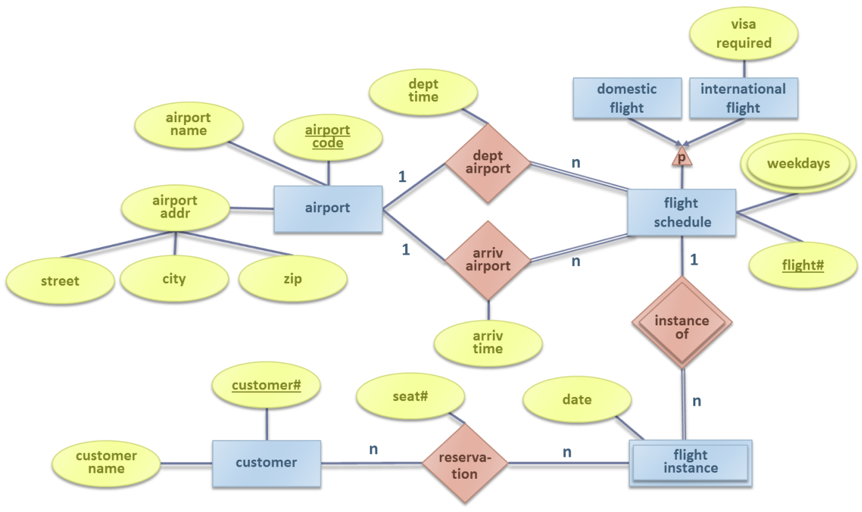
\includegraphics[width=\linewidth]{entities.png}
  \caption{Διάγραμμα Οντοτήτων/Συσχετίσεων}
\end{figure}


%%% Local Variables:
%%% mode: latex
%%% TeX-master: "main"
%%% End:

  
\section{Σχεσιακό μοντέλο}

\subsection{Πεδία ορισμού}


\begin{tabular}{|p{6cm}|p{8cm}|}
\hline
  \textbf{Πεδίο Ορισμού} & \textbf{Τύπος}         \\ \hline
  Ακέραιος               & INT                    \\ \hline
  Όνομα                  & VARCHAR(40)            \\ \hline
  Δυαδικό                & ENUMERATED\{Ναι, Όχι\} \\ \hline
  Εκδηλώσεις             & ENUMERATED\{Εκδήλωση, Μουσική Εκδήλωση, Θεατρική
                  Εκδήλωση, Αθλητική Εκδήλωση\}   \\ \hline
  Κείμενο                & VARCHAR(140)           \\ \hline
  Διεύθυνση              & VARCHAR(35)            \\ \hline
  Ώρα                    & TIME                   \\ \hline
  Ημερομηνία             & DATE                   \\ \hline
  Τηλεφωνο               & VARCHAR(14)            \\ \hline
  Τιμή                   & DEC(2,2)               \\ \hline
  email                  & VARCHAR(30)            \\ \hline
  pass                   & VARCHAR(15)            \\ \hline
  Αριθμός16              & DEC(16,0)              \\ \hline
  Αριθμός3               & DEC(3,0)               \\ \hline
  Εισιτήρια              & VARCHAR(10)            \\ \hline
\end{tabular}

\subsection{Σχέσεις}

Παρακάτω παρουσιάζονται οι σχέσεις της EventsDB, όπως μεταφέρονται από
το μοντέλο οντοτήτων/ συσχετίσεων στην τρίτη κανονική τους μορφή.

\subsubsection*{Εκδήλωση}

\begin{tabular}{|p{6cm}|p{8cm}|}
  \multicolumn{2}{l}{\textbf{Γνωρίσματα:}}                         \\ \hline
  Όνομα                   & Τύπος                                  \\ \hline
  Κωδικός\_εκδήλωσης      & Ακέραιος                               \\ \hline
  Όνομα\_εκδήλωσης        & Όνομα                                  \\ \hline
  Τύπος                   & Εκδηλώσεις                             \\ \hline
  Κοινό\_που\_απευθύνεται & Όνομα                                  \\ \hline
  Περιγραφή               & Κείμενο                                \\ \hline
  Ημερομηνία              & Ημερομηνία                             \\ \hline
  Ώρα\_έναρξης            & Ώρα                                    \\ \hline
  Κωδικός\_τοπεθεσίας     & Ακέραιος                               \\ \hline
  Κωδικός\_ερμηνευτή      & Ακέραιος                               \\ \hline
  Κωσικός\_διοργανωτή     & Ακέραιος                               \\ \hline
  \multicolumn{2}{l}{\textbf{Περιορισμοί Ακεραιότητας:}}           \\ \hline
  Πρωτεύον Κλειδί         & Κωδικός\_εκδήλωσης                     \\ \hline
  Ξένα Κλειδιά            & Κωδικός\_τοποθεσίας -> Τοποθεσία       \\ \cline{2-2}
                          & Κωδικός\_Ερμηνευτή -> Καλλιτέχνης-Ομάδα \\ \cline{2-2}
                          & Κωδικός\_διοργανώτή -> Διοργανωτής     \\ \hline
\end{tabular}

\subsubsection*{Μουσική\_εκδήλωση}

\begin{tabular}{|p{6cm}|p{8cm}|}
  \multicolumn{2}{l}{\textbf{Γνωρίσματα:}}                   \\ \hline
  Όνομα                     & Τύπος                          \\ \hline
  Κωδικός\_εκδήλωσης        & Ακέραιος                       \\ \hline
  Ύπαρξη\_θέσεων\_καθημένων & Διαδικό                        \\ \hline
  Είδος                     & Κείμενο                        \\ \hline
  Opening\_act              & Κείμενο                        \\ \hline
  \multicolumn{2}{l}{\textbf{Περιορισμοί Ακεραιότητας:}}     \\ \hline
  Πρωτεύον Κλειδί           & Κωδικός\_εκδήλωσης             \\ \hline
  Ξένα Κλειδιά              & Κωδικός\_εκδήλωσης -> Εκδήλωση \\ \hline
\end{tabular}

\subsubsection*{Θέατρο}

\begin{tabular}{|p{6cm}|p{8cm}|}
  \multicolumn{2}{l}{\textbf{Γνωρίσματα:}}               \\ \hline
  Όνομα               & Τύπος                            \\ \hline
  Κωδικός\_εκδήλωσης  & Ακέραιος                         \\ \hline
  Ύπαρξη\_θέσεων\_VIP & Διαδικό                          \\ \hline
  Διάρκεια            & Ακέραιος                         \\ \hline
  \multicolumn{2}{l}{\textbf{Περιορισμοί Ακεραιότητας:}} \\ \hline
  Πρωτεύον Κλειδί     & Κωδικός\_εκδήλωσης               \\ \hline
  Ξένα Κλειδιά        & Κωδικός\_εκδήλωσης -> Εκδήλωση   \\ \hline
\end{tabular}

\subsubsection*{Αθλητική\_εκδήλωση}

\begin{tabular}{|p{6cm}|p{8cm}|}
  \multicolumn{2}{l}{\textbf{Γνωρίσματα:}}               \\ \hline
  Όνομα               & Τύπος                            \\ \hline
  Κωδικός\_εκδήλωσης  & Ακέραιος                         \\ \hline
  Ύπαρξη\_θέσεων\_VIP & Δυαδικό                          \\ \hline
  Άθλημα              & Κείμενο                          \\ \hline
  \multicolumn{2}{l}{\textbf{Περιορισμοί Ακεραιότητας:}} \\ \hline
  Πρωτεύον Κλειδί     & Κωδικός\_εκδήλωσης               \\ \hline
  Ξένα Κλειδιά        & Κωδικός\_εκδήλωσης -> Εκδήλωση   \\ \hline
\end{tabular}

\subsubsection*{Εισιτήριο}

\begin{tabular}{|p{6cm}|p{8cm}|}
  \multicolumn{2}{l}{\textbf{Γνωρίσματα:}}                     \\ \hline
  Όνομα              & Τύπος                                   \\ \hline
  Κωδικός\_εκδήλωσης & Ακέραιος                                \\ \hline
  Τύπος\_εισιτηρίου  & Εισιτήρια                               \\ \hline
  Τιμή               & Τιμή                                    \\ \hline
  \multicolumn{2}{l}{\textbf{Περιορισμοί Ακεραιότητας:}}       \\ \hline
  Πρωτεύον Κλειδί    & Κωδικός\_εκδήλωσης \& Τύπος\_εισιτηρίου \\ \hline
  Ξένο Κλειδί        & Κωδικός\_εκδήλωσης -> Εκδήλωση          \\ \hline
\end{tabular}


\subsubsection*{Τοποθεσία}

\begin{tabular}{|p{6cm}|p{8cm}|}
  \multicolumn{2}{l}{\textbf{Γνωρίσματα:}}               \\ \hline
  Όνομα                  & Τύπος                         \\ \hline
  Κωδικός\_τοποθεσίας    & Ακέραιος                      \\ \hline
  Όνομα\_τοποθεσίας      & Όνομα                         \\ \hline
  Εσωτερικός\_χώρος      & Δυαδικό                       \\ \hline
  Τηλέφωνο               & Τηλέφωνο                      \\ \hline
  Διεύθυνση              & Διεύθυνση                     \\ \hline
  Ύπαρξη\_υποδομών\_ΑΜΕΑ & Δυαδικό                       \\ \hline
  Τιμή\_μπύρας           & Τιμή                          \\ \hline
  Τιμή\_κρασιού          & Τιμή                          \\ \hline
  Τιμή\_Ποτού            & Τιμή                          \\ \hline
  \multicolumn{2}{l}{\textbf{Περιορισμοί Ακεραιότητας:}} \\ \hline
  Πρωτεύον Κλειδί        & Κωδικός\_τοποθεσίας           \\ \hline
\end{tabular}


\subsubsection*{Καλλιτέχνης-Ομάδα}

\begin{tabular}{|p{6cm}|p{8cm}|}
  \multicolumn{2}{l}{\textbf{Γνωρίσματα:}}               \\ \hline
  Όνομα              & Τύπος                             \\ \hline
  Κωδικός\_ερμηνευτή & Ακέραιος                          \\ \hline
  Ονοματεπώνυμο      & Όνομα                             \\ \hline
  Καταγωγή           & Όνομα                             \\ \hline
  \multicolumn{2}{l}{\textbf{Περιορισμοί Ακεραιότητας:}} \\ \hline
  Πρωτεύον Κλειδί    & Κωδικός\_ερμηνευτή                \\ \hline
\end{tabular}

\subsubsection*{Καλλιτέχνης}

\begin{tabular}{|p{6cm}|p{8cm}|}
  \multicolumn{2}{l}{\textbf{Γνωρίσματα:}}                       \\ \hline
  Όνομα                & Τύπος                                   \\ \hline
  Κωδικός\_ερμηνευτή   & Ακέραιος                                \\ \hline
  Είδος                & Όνομα                                   \\ \hline
  Ημερομηνία\_γέννησης & Ημερομηνία                              \\ \hline
  \multicolumn{2}{l}{\textbf{Περιορισμοί Ακεραιότητας:}}         \\ \hline
  Πρωτεύον Κλειδί      & Κωδικός\_ερμηνευτή                      \\ \hline
  Ξένο Κλειδί          & Κωδικός\_ερμηνευτή -> Καλλιτέχνης-Ομάδα \\ \hline
\end{tabular}

\subsubsection*{Ομάδα}

\begin{tabular}{|p{6cm}|p{8cm}|}
  \multicolumn{2}{l}{\textbf{Γνωρίσματα:}}                     \\ \hline
  Όνομα              & Τύπος                                   \\ \hline
  Κωδικός\_ερμηνευτή & Ακέραιος                                \\ \hline
  Όνομα\_υπευθύνου   & Όνομα                                   \\ \hline
  \multicolumn{2}{l}{\textbf{Περιορισμοί Ακεραιότητας:}}       \\ \hline
  Πρωτεύον Κλειδί    & Κωδικός\_ερμηνευτή                      \\ \hline
  Ξένο Κλειδί        & Κωδικός\_ερμηνευτή -> Καλλιτέχνης-Ομάδα \\ \hline
\end{tabular}


\subsubsection*{Φυσικό\_σημείο\_προπώλησης}

\begin{tabular}{|p{6cm}|p{8cm}|}
  \multicolumn{2}{l}{\textbf{Γνωρίσματα:}}               \\ \hline
  Όνομα            & Τύπος                               \\ \hline
  Κωδικός\_σημείου & Ακέραιος                            \\ \hline
  Όνομα\_σημείου   & Όνομα                               \\ \hline
  Τηλέφωνο         & Τηλέφωνο                            \\ \hline
  Διεύθυνση        & Διεύθυνση                           \\ \hline
  \multicolumn{2}{l}{\textbf{Περιορισμοί Ακεραιότητας:}} \\ \hline
  Πρωτεύον Κλειδί  & Κωδικός\_σημείου                    \\ \hline
\end{tabular}

\subsubsection*{Προπώληση}

\begin{tabular}{|p{6cm}|p{8cm}|}
  \multicolumn{2}{l}{\textbf{Γνωρίσματα:}}                    \\ \hline
  Όνομα              & Τύπος                                  \\ \hline
  Κωδικός\_σημείου   & Ακέραιος                               \\ \hline
  Κωδικός\_εκδήλωσης & Ακέραιος                               \\ \hline
  Πρωτεύον Κλειδί    & Κωδικός\_σημείου \& Κωδικός\_εκδήλωσης \\ \hline
  Ξένο Κλειδί        & Κωδικός\_σημείου -> Φυσικό\_σημείο\_προπώλησης
                                                              \\ \hline
                     & Κωδικός\_εκδήλωσης -> Εκδήλωση         \\ \hline
\end{tabular}


\subsubsection*{Διοργανωτής}

\begin{tabular}{|p{6cm}|p{8cm}|}
  \multicolumn{2}{l}{\textbf{Γνωρίσματα:}}               \\ \hline
  Όνομα               & Τύπος                            \\ \hline
  Κωδικός\_διοργανωτή & Ακέραιος                         \\ \hline
  Όνομα\_εταιρίας     & Όνομα                            \\ \hline
  email               & email                            \\ \hline
  Τηλέφωνο            & Τηλέφωνο                         \\ \hline
  password            & pass                             \\ \hline
  \multicolumn{2}{l}{\textbf{Περιορισμοί Ακεραιότητας:}} \\ \hline
  Πρωτεύον Κλειδί     & Κωδικός\_διοργανωτή              \\ \hline
\end{tabular}


\subsubsection*{Χρήστης}

\begin{tabular}{|p{6cm}|p{8cm}|}
  \multicolumn{2}{l}{\textbf{Γνωρίσματα:}}               \\ \hline
  Όνομα           & Τύπος                                \\ \hline
  Κωδικός\_χρήστη & Ακέραιος                             \\ \hline
  Ονοματεπώνυμο   & Όνομα                                \\ \hline
  email           & email                                \\ \hline
  password        & pass                                 \\ \hline
  \multicolumn{2}{l}{\textbf{Περιορισμοί Ακεραιότητας:}} \\ \hline
  Πρωτεύον Κλειδί & Κωδικός\_χρήστη                      \\ \hline
\end{tabular}


\subsubsection*{Κάρτα}

\begin{tabular}{|p{6cm}|p{8cm}|}
  \multicolumn{2}{l}{\textbf{Γνωρίσματα:}}               \\ \hline
  Όνομα              & Τύπος                             \\ \hline
  Αριθμός\_κάρτας    & Αριθμός16                         \\ \hline
  Αριθμός\_ασφαλείας & Αριθμός3                          \\ \hline
  Διεύθυνση          & Διεύθυνση                         \\ \hline
  Κωδικός\_χρήστη    & Ακέραιος                          \\ \hline
  \multicolumn{2}{l}{\textbf{Περιορισμοί Ακεραιότητας:}} \\ \hline
  Πρωτεύον Κλειδί    & Αριθμός\_κάρτας                   \\ \hline
  Ξένα Κλειδιά       & Κωδικός\_χρήστη -> Χρήστης        \\ \hline
\end{tabular}

\subsubsection*{Αγορά}

\begin{tabular}{|p{6cm}|p{8cm}|}
  \multicolumn{2}{l}{\textbf{Γνωρίσματα:}}                   \\ \hline
  Όνομα              & Τύπος                                 \\ \hline
  Κωδικός\_εκδήλωσης & Ακέραιος                              \\ \hline
  Κωδικός\_χρήστη    & Ακέραιος                              \\ \hline
  Τύπος\_εισιτηρίου  & Εισιτήρια                             \\ \hline
  \multicolumn{2}{l}{\textbf{Περιορισμοί Ακεραιότητας:}}     \\ \hline
  Πρωτεύον Κλειδί    & Κωδικός\_χρήστη \& Κωδικός\_εκδήλωσης \\ \hline
  Ξένα Κλειδιά       & Κωδικός\_χρήστη -> Χρήστης            \\ \hline
                     & Κωδικός\_εκδήλωσης -> Εκδήλωση        \\ \hline
\end{tabular}

\subsubsection*{Ενδιαφέρον}

\begin{tabular}{|p{6cm}|p{8cm}|}
  \multicolumn{2}{l}{\textbf{Γνωρίσματα:}}                   \\ \hline
  Όνομα              & Τύπος                                 \\ \hline
  Κωδικός\_εκδήλωσης & Ακέραιος                              \\ \hline
  Κωδικός\_χρήστη    & Ακέραιος                              \\ \hline
  \multicolumn{2}{l}{\textbf{Περιορισμοί Ακεραιότητας:}}     \\ \hline
  Πρωτεύον Κλειδί    & Κωδικός\_χρήστη \& Κωδικός\_εκδήλωσης \\ \hline
  Ξένα Κλειδιά       & Κωδικός\_χρήστη -> Χρήστης            \\ \hline
                     & Κωδικός\_εκδήλωσης -> εκδήλωση        \\ \hline
\end{tabular}

\subsection{Σχεσιακό Σχήμα}

\begin{figure}[H]
  \centering
  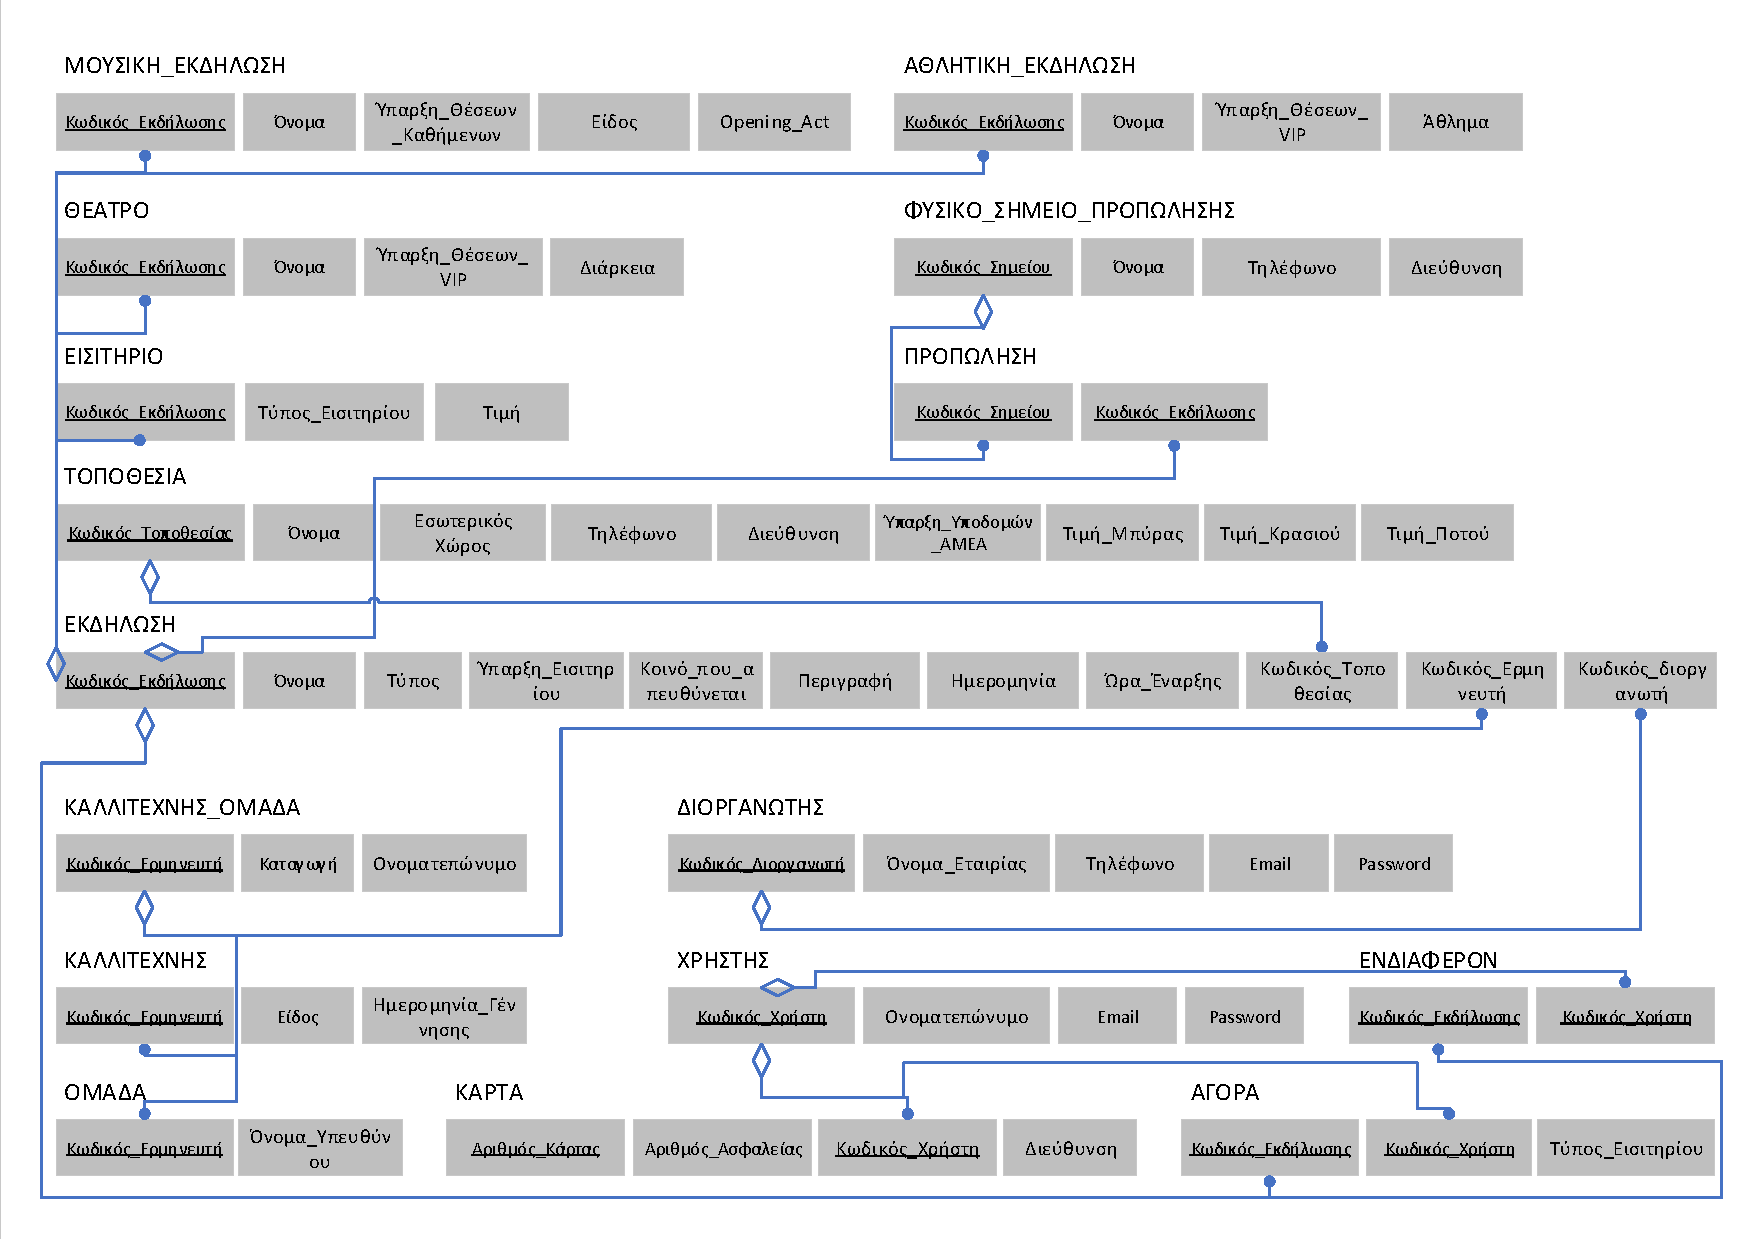
\includegraphics[width=\linewidth]{Relations.pdf}
  \caption{Σχεσιακό μοντέλο}
\end{figure}

\subsection{Όψεις}

Παρακάτω παρουσιάζονται κάποιες ενδεικτικές όψεις της βάσης δεδομένων
οι οποίες δίνουν μια πολύ καλή εικόνα για το πως όλες οι σχέσεις
συνδέονται μεταξύ τους. Αρκετές όψεις έχουν πολλές ομοιότητες μεταξύ
τους και γι' αυτόν τον λόγο θα παρουσιαστούν ενδεικτικά κάποιες από
αυτές.


%%% Local Variables:
%%% mode: latex
%%% TeX-master: "main"
%%% TeX-engine: xetex
%%% End:

  \section{Παραδείγματα}

\subsection{Παραδείγματα Πινάκων}

Παράδειγμα για τον πίνακα Μουσική\_Εκδήλωση της EventsDB:

\begin{table}[H]
  \centering
  \footnotesize
\begin{tabular}[c]{|p{2cm}|p{2.5cm}|p{2.5cm}|p{2cm}|p{3.5cm}|}
  \hline
  Κωδικός\_ Εκδήλωσης & Όνομα                           & Ύπαρξη\_Θέσεων\_ Καθήμενων & Είδος                       & Opening\_Act            \\ \hline
  8053                & Ημισκούμπρια - 23rd Anniversary Live & Όχι                         & Hip hop Live                & DJ Πρύτανης warm up set \\ \hline
  8055                & Συναυλία Θάνου Μικρούτσικου     & Όχι                         & Έντεχνο τραγούδι - Συναυλία & Μίλτος Πασχαλίδης       \\ \hline
\end{tabular}
\end{table}

Εκτίμηση για τον αριθμό των εγγραφών: \textasciitilde 40000

Παράδειγμα για τον πίνακα Αθλητική\_Εκδήλωση της EventsDB:

\begin{table}[H]
  \centering
  \footnotesize
  \begin{tabular}{|p{3cm}|p{4cm}|p{3cm}|p{3cm}|}
  \hline
  Κωδικός\_Εκδήλωσης & Όνομα & Ύπαρξη\_Θέσεων\_VIP & Άθλημα \\ \hline
  4444 & Τελικός Πρωταθλήματος ΠΑΟΚ - Παναθηναϊκός & Ναι & Μπάσκετ \\ \hline
  1235 & Προβολή Live Τελικού Roldand Garros & Ναι & Τένις \\ \hline
  6969 & Manos' Beerpong Challenge X Erasmus & Όχι & Beerpong \\ \hline
\end{tabular}
\end{table}
  
Εκτίμηση για τον αριθμό των εγγραφών: \textasciitilde 40000

Παράδειγμα για τον πίνακα Θέατρο της EventsDB:

\begin{table}[H]
  \centering
  \footnotesize
  \begin{tabular}{|p{3cm}|p{4cm}|p{3cm}|p{3cm}|}
  \hline
  Κωδικός\_Εκδήλωσης & Όνομα & Ύπαρξη\_Θέσεων\_VIP & Διάρκεια \\ \hline
  7777 & Οι Βάκχες του Ευρυπίδη & Όχι & 114 \\ \hline
  0666 & Stand up Comedy by George Carlin & Ναι & 74 \\ \hline
\end{tabular}
\end{table}
  
Εκτίμηση για τον αριθμό των εγγραφών: \textasciitilde 40000

Παράδειγμα για τον πίνακα Εισιτήριο της EventsDB:

\begin{table}[H]
  \centering
  \footnotesize
  \begin{tabular}{|c|c|c|}
  \hline
  Κωδικός\_Εκδήλωσης & Τύπος\_Εισιτηρίου & Τιμή \\ \hline
  7777 & Φοιτητικό & 14 \\ \hline
  7777 & Ενηλίκων & 28 \\ \hline
  8053 & Ενηλίκων & 12 \\ \hline
  8055 & Φοιτητικό & 14 \\ \hline
  8055 & Ενηλίκων & 18 \\ \hline
  4444 & Ενηλίκων & 10 \\ \hline
  1235 & Ενηλίκων & 4 \\ \hline
  0666 & Ενηλίκων & 30 \\ \hline
  0666 & Υπερήλικων & 20 \\ \hline
  6969 & Ενηλίκων & 5 \\ \hline
\end{tabular}
\end{table}
  
Εκτίμηση για τον αριθμό των εγγραφών: \textasciitilde 40000

Παράδειγμα για τον πίνακα Φυσικό\_Σημείο\_Προπώλησης της EventsDB:

\begin{table}[H]
  \centering
  \footnotesize
  \begin{tabular}{|p{3cm}|p{4cm}|p{3cm}|p{3cm}|}
  \hline
  Κωδικός\_Σημείου & Όνομα & Τηλέφωνο & Διεύθυνση \\ \hline
  12345 & Καταστήματα Public Τσιμισκή & 2310227288 & Τσιμισκή 24 \\ \hline
  14310 & Γραμματεία Τμήματος ΗΜΜΥ - Σούλα Γκλάμουρους & 2310 666 666 & Θεσσαλονίκη 54124 \\ \hline
\end{tabular}
\end{table}
  
Εκτίμηση για τον αριθμό των εγγραφών: \textasciitilde 40000

Παράδειγμα για τον πίνακα Προπώληση της EventsDB:

\begin{table}[H]
  \centering
  \footnotesize
  \begin{tabular}{|c|c|}
  \hline
  Κωδικός\_Σημείου & Κωδικός\_Εκδήλωσης \\ \hline
  12345 & 7777 \\ \hline
  12345 & 0666 \\ \hline
  12345 & 8053 \\ \hline
  12345 & 8055 \\ \hline
  14310 & 4444 \\ \hline
  14310 & 1235 \\ \hline
  14310 & 6969 \\ \hline
\end{tabular}
\end{table}
  
Εκτίμηση για τον αριθμό των εγγραφών: \textasciitilde 40000

Παράδειγμα για τον πίνακα Τοποθεσία της EventsDB:

\begin{table}[H]
  \centering
  \footnotesize
  \begin{tabular}{|p{1.8cm}|p{2cm}|p{1.6cm}|p{1.6cm}|p{2.5cm}|l}
  \hline
  Κωδικός\_Τοποθεσίας & Όνομα & Εσωτερικός\_ Χώρος & Τηλέφωνο & Διεύθυνση
    & \ldots \\ \hline
  132435 & WE - Sports \& culture facility & Ναι & 2310284700 & 3ης Σεπτεμβρίου 3 & \ldots \\ \hline
  532413 & Paok Sports Arena & Ναι & 2310192600 & Πυλαία-Χορτιάτης 555 35 &\ldots \\ \hline
  \end{tabular}
  \begin{tabular}{r|p{2cm}|p{2cm}|p{2cm}|p{2cm}|}
  \hline
    \ldots & Ύπαρξη\_ Υποδομών\_ΑΜΕΑ & Τιμή\_ Μπύρας & Τιμή\_ Κρασιού
    & Τιμή\_ Ποτού \\ \hline
    \ldots & Όχι & 4 & 6 & 7 \\ \hline
    \ldots & Ναι & NULL & NULL & NULL \\ \hline
\end{tabular}
\end{table}
  
Εκτίμηση για τον αριθμό των εγγραφών: \textasciitilde 40000

Παράδειγμα για τον πίνακα Εκδήλωση της EventsDB:

\begin{table}[H]
  \centering
  \footnotesize
  \begin{tabular}{|p{1.6cm}|p{2.8cm}|p{1.5cm}|l|l|l}
  \hline
  Κωδικός\_ Εκδήλωσης & Όνομα                               
    & Ύπαρξη\_ Εισιτηρίου & Κοινό              & Περιγραφή & \ldots \\ \hline
  6969               & Manos' Beerpong Challenge X Erasmus 
    & Ναι                & Θαρραλέοι Φοιτητές & Try to not get
                                                shitfaced & \ldots  \\ \hline
  8053               & Ημισκούμπρια - 23rd Anniversary Live
    & Ναι            & Χιουμορίστες και Χιπχοπάδες & Πάμε όλοι μαζί σε μια παραλία & \ldots  \\ \hline
  8055               & Συναυλία Θάνου Μικρούτσικου & Ναι
    & Ελεύθεροι και χωρισμένοι & Συναυλία & \ldots  \\ \hline
  4444               & Τελικός Πρωταθλήματος ΠΑΟΚ - Παναθηναϊκός
    & Ναι            & Άρρωστα παόκια κυρίως & Μην τα σπάσετε όλα όλα & \ldots \\hline
  1235               & Προβολή Live Τελικού Roldand Garros 
    & Ναι            & Φίλοι Αντισφαίρισης & Μπύρες στη μισή τιμή   \\ \hline
  7777               & Οι Βάκχες του Ευρυπίδη & Ναι
    & Ψαγμένα τυπάκια & Λε κουλτουρ Υψηλό & \ldots \\ \hline
  0666               & Stand up Comedy by George Carlin
    & Ναι            & Μη παρεξηγησιάρηδες & One Last HBO Special & \ldots \\ \hline
  \end{tabular}
   \begin{tabular}{r|l|l|l|l|l|}
  \hline
  \ldots & Ημερομηνία         & Ώρα\_Έναρξης & Κωδικός\_Τοποθεσίας & Κωδικός\_Ερμηνευτή & Κωδικός\_Διοργανωτή \\ \hline
  \ldots & 23 Δεκεμβρίου 2018 & 21:00        & 132435              & NULL               & 72150               \\ \hline
  \ldots & 20 Μαρτίου 2019    & 21:00        & 532413              & 122333             & 11888               \\ \hline
  \ldots & 18 Ιουνίου 2019    & 20:30        & 532413              & 555551             & 11888               \\ \hline
  \ldots & 10 Μαρτίου 2019    & 19:30        & 532413              & 444444             & 11888               \\ \hline
  \ldots & 29 Μαϊου 2019      & 16:30        & 132435              & NULL               & 72150               \\ \hline
  \ldots & 19 Δεκέμβρη 2018   & 20:30        & 532413              & 192837             & 11888               \\ \hline
  \ldots & 25 Μαρτίου 2019    & 00:00        & 532413              & 382957             & 72510               \\ \hline
\end{tabular}
\end{table}
  
Εκτίμηση για τον αριθμό των εγγραφών: \textasciitilde 40000

Παράδειγμα για τον πίνακα Καλλιτέχνης\_Ομάδα της EventsDB:

\begin{table}[H]
  \centering
  \footnotesize
  \begin{tabular}{|l|l|l|}
  \hline
  Κωδικός\_Ερμηνευτή & Καταγωγή & Ονοματεπώνυμο \\ \hline
  122333 & Αθήνα - Ελλάδα & Μετζέλος, Μιρθιδάτης, Dj Πρύτανης \\ \hline
  555551 & Ελλάδα & Θάνος Μικρούτσικος \\ \hline
  444444 & Ελλάδα & Ομάδα Μπάσκετ Ενηλίκων ΠΑΟΚ \\ \hline
  382957 & USA cemetery & George Carlin's Ghost  \\ \hline
  192837 & Ελλάδα & Ανώτερη Δραματική Σχολή Θεσσαλονίκης \\ \hline
\end{tabular}
\end{table}
  
Εκτίμηση για τον αριθμό των εγγραφών: \textasciitilde 40000

Παράδειγμα για τον πίνακα καλλιτέχνης της EventsDB:

\begin{table}[H]
  \centering
  \footnotesize
  \begin{tabular}{|l|l|l|}
  \hline
  Κωδικός\_Ερμηνευτή & Είδος & Ημερομηνία\_Γέννησης \\ \hline
  555551 & Έντεχνο & 1947 \\ \hline
  122333 & Ελληνικό Hip Hop & 1975 \\ \hline
\end{tabular}
\end{table}
  
Εκτίμηση για τον αριθμό των εγγραφών: \textasciitilde 40000

Παράδειγμα για τον πίνακα Ομάδα της EventsDB:

\begin{table}[H]
  \centering
  \footnotesize
  \begin{tabular}{|l|l|}
  \hline
  Κωδικός\_Ερμηνευτή & Όνομα\_Υπευθύνου \\ \hline
  444444 & Ιβάν Σαββίδης \\ \hline
  382957 & Ηλίας Ψινάκης \\ \hline
  192837 & Ανδρέας Βουτσινάς \\ \hline
\end{tabular}
\end{table}
  
Εκτίμηση για τον αριθμό των εγγραφών: \textasciitilde 40000

Παράδειγμα για τον πίνακα Διοργανωτής της EventsDB:

\begin{table}[H]
  \centering
  \footnotesize
  \begin{tabular}{|l|l|l|l|l|}
  \hline
  Κωδικός\_Διοργανωτή & Όνομα\_Εταιρίας & Τηλέφωνο & Email & Password \\ \hline
  72150 & Party Animal Events & 6981811474 & manoszisis@yahoo.gr & 3ebb9abf12d5b17\ldots \\ \hline
  11888 & Culture AE @ 6979695949 & og34582@mhrit.net & 2p3oroh2c3ri23i\ldots \\ \hline
\end{tabular}
\end{table}
  
Εκτίμηση για τον αριθμό των εγγραφών: \textasciitilde 40000

Παράδειγμα για τον πίνακα Χρήστης της EventsDB:

\begin{table}[H]
  \centering
  \footnotesize
  \begin{tabular}{|l|l|l|l|}
  \hline
  Κωδικός\_Χρήστη & Ονοματεπώνυμο & Email & Password \\ \hline
  006689 & Φρανγκίσκος Μπλανίνγκιος & pinkypromises@gmail.com &
                                                                82a545b150da45c\ldots \\ \hline
  008055 & Χρυσηίδα Τοντόροβιτς & cultureoverload@gmail.com & 2cur239vj293d\ldots \\ \hline
\end{tabular}
\end{table}
  
Εκτίμηση για τον αριθμό των εγγραφών: \textasciitilde 40000

Παράδειγμα για τον πίνακα Κάρτα της EventsDB:

\begin{table}[H]
  \centering
  \footnotesize
  \begin{tabular}{|l|l|l|l|}
  \hline
  Αριθμός\_Κάρτας & Αριθμός\_Ασφαλείας & Κωδικός\_Χρήστη & Διεύθυνση \\ \hline
  1234 5678 9999 & 489 & 006689 & Προβληματικού 6 \\ \hline
  9999 8765 4321 & 987 & 008055 & κωμωδίας 21 \\ \hline
\end{tabular}
\end{table}
  
Εκτίμηση για τον αριθμό των εγγραφών: \textasciitilde 40000

Παράδειγμα για τον πίνακα Αγορά της EventsDB:

\begin{table}[H]
  \centering
  \footnotesize
  \begin{tabular}{|l|l|l|}
  \hline
  Κωδικός\_Εκδήλωσης & Κωδικός\_Χρήστη & Τύπος\_Εισιτηρίου \\ \hline
  0666 & 006689 & Υπερήλικων \\ \hline
  8055 & 008055 & Εφηβικό \\ \hline
  6969 & 006689 & Ενηλίκων \\ \hline
  4444 & 008055 & Ενηλίκων \\ \hline
  
\end{tabular}
\end{table}
  
Εκτίμηση για τον αριθμό των εγγραφών: \textasciitilde 40000

Παράδειγμα για τον πίνακα Ενδιαφέρον της EventsDB:

\begin{table}[H]
  \centering
  \footnotesize
  \begin{tabular}{|l|l|}
  \hline
  Κωδικός\_Εκδήλωσης & Κωδικός\_Χρήστη \\ \hline
  4444 & 008055 \\ \hline
  1235 & 006689 \\ \hline
  6969 & 006689 \\ \hline
  0666 & 006689 \\ \hline
  8055 & 008055 \\ \hline
\end{tabular}
\end{table}
  
Εκτίμηση για τον αριθμό των εγγραφών: \textasciitilde 40000

\subsection{Παραδείγματα Ερωτημάτων}

Τα κυριότερα ερωτήματα αφορούν την προβολή στοιχείων εκδηλώσεων με
διάφορα κριτήρια. Οποιοσδήποτε συνδυασμός γνωρισμάτων μπορεί να
προβληθεί. Στην παρακάτω περίπτωση θα προβληθεί μόνο το όνομα της
εκδήλωσης, η ημερομηνία και είτε το όνομα της τοποθεσίας διεξαγωγής
είτε το όνομα του καλλιτέχνη.  Κάποια κριτήρια αναζήτησής εκδηλώσεων
είναι βάση του ονόματος του τοποθεσίας (\ref{eq1}), όνομα του
καλλιτέχνη (\ref{eq2}), ή συγκεκριμένου τύπου εκδήλωσης (\ref{eq3}).

\begin{equation} \label{eq1}
\begin{split}
&A \leftarrow \text{Εκδήλωση} \bowtie
\text{Καλλιτέχνης-Ομάδα} \bowtie
\sigma_{<\text{Όνομα\_τοποθεσίας} = \text{"Τα Ξύδια"}>}
\text{Τοποθεσία}
\\
&\Pi_{<\text{Όνομα\_εκδήλωσης, Ημερομηνία,Ονοματεπώνυμο}>}A
\end{split}
\end{equation}

\begin{equation} \label{eq2}
\begin{split}
&A \leftarrow \text{Εκδήλωση} \bowtie
\text{Τοποθεσία} \bowtie
\sigma_{<\text{Ονοματεπώνυμο} = \text{"Γιάννης Μπουζούκης"}>}
\text{Καλλιτέχνης-Ομάδα}
\\
&\Pi_{<\text{Όνομα\_εκδήλωσης, Ημερομηνία,Όνομα\_Τοποθεσίας}>}A
\end{split}
\end{equation}

\begin{equation} \label{eq3}
\begin{split}
&A \leftarrow \text{Καλλιτέχνης-Ομάδα} \bowtie
\sigma_{<\text{Τύπος} = \text{"Μουσική εκδήλωση"}>}\text{Εκδήλωση}
\\
&\Pi_{<\text{Όνομα\_εκδήλωσης, Ημερομηνία, Ονοματεπώνυμο}>}A
\end{split}
\end{equation}

Ένα εξίσου σημαντικό ερώτημα  είναι η αναζήτηση μια εκδήλωσης βάση της
ημέρας διεξαγωγής. Είτε για μία συγκεκριμένη ημερομηνία και ώρα είτε
για ένα εύρος (\ref{eq4}).

\begin{equation}
  \label{eq4}
  \begin{split}
    &\Pi_{<\text{Όνομα\_εκδήλωσης, Ημερομηνία, Ονοματεπώνυμο}>}(
    \sigma_{<\text{Ημερομηνία} = 23/11/2018>} \text{Εκδήλωση} \bowtie
    \text{Καλλιτέχνης-Ομάδα})
  \end{split}
\end{equation}

Πέρα από τα ερωτήματά όπου αφορά τα στοιχεία των εκδηλώσεων, ένα
σημαντικό ερώτημά, αναγκαίο για την ολοκλήρωση της παροχής υπηρεσιών
αγοράς εισιτήριων, είναι η προβολή όλων των χρηστών όπου έχουν
πραγματοποιήσει αγορά κάποιου εισιτηρίου για μια συγκεκριμένη εκδήλωση
(\ref{eq5}). Αυτό θα είναι διαθέσιμη μόνο στον χρήστη Διοργανωτής ο
οποίος συσχετίζεται με την εκάστοτε εκδήλωση.

\begin{equation}
  \label{eq5}
  \begin{split}
    &\Pi_{<\text{Ονοματεπώνυμο, Τύπος\_εισιτηρίου}>}(
    \sigma_{<\text{Κωδικός\_εκδήλωσης} = 42>} \text{Αγορά} \bowtie
    \text{Χρήστης})
  \end{split}
\end{equation}

Τέλος, παρουσιάζεται ένα ακόμα ερώτημα το οποίο αφορά τον χρήστη
Εγγεγραμμένος Χρήστης ο οποίος θα θελήσει να προβάλει όλες τις
αποθηκευμένες του εκδηλώσεις . (\ref{eq6}).


\begin{equation}
  \label{eq6}
  \begin{split}
    &A \leftarrow \sigma_{<\text{Κωδικός\_χρήστη} = 8055>}
    \text{Ενδιαφέρον} \bowtie \text{Εκδήλωση} \bowtie \text{Τοποθεσία}
    \bowtie \text{Καλλιτέχνης-Ομάδα} \\
    &\Pi_{<\text{Όνομα, Ημερομηνία, Ώρα\_έναρξης, Όνομα\_τοποθεσίας,
        Ονοματεπώνυμο}>}A
  \end{split}
\end{equation}



% (Δώστε ενδεικτικά παραδείγματα χρήσιμων ερωτημάτων.)

% Παράδειγμα για τη FlightsDB:

% έστω οι σχέσεις:

% \begin{itemize}[noitemsep]
% \item CUSTOMER(cust\_id, firstname, lastname, phone, street, city,
%   zip)
% \item RESERVATION(flight\_id, date, cust\_id, ticket\_no, seat\_no)
% \end{itemize}

% Για μια πτήση (έστω την AA101) υποθέτουμε ότι ο/η αεροσυνοδός θα ήθελε
% να έχει τη λίστα των επιβατών μαζί με χρήσιμες πληροφορίες για το
% check in (id επιβάτη, αριθμός εισιτηρίου, θέση, όνομα και επώνυμο για
% κάθε επιβάτη). Εκτελούμε το παρακάτω ερώτημα:

% πticket\_no, seat\_no, cust\_id(σflight\_id=AA101(RESERVATION))
% πcust\_id, firstname, lastname(CUSTOMER)


%%% Local Variables:
%%% mode: latex
%%% TeX-master: "main"
%%% TeX-engine: xetex
%%% End:


  % \bibliographystyle{ieeetr}
  % \bibliography{cites}{}
  % \bibliographystyle{plain}

\end{document}
%%% Local Variables:
%%% mode: latex
%%% TeX-master: t
%%% TeX-engine: xetex
%%% End:
